%
\chapter{Varying CoM Height}%
\label{chap:varyingheight}
As mentioned earlier, recently work has been done in removing the constant height assumption from the walking model. The motivation for this is threefold. The use of height can be used in tracking control. Where angular momentum and the \ac{CoP} are often the two control inputs for a \ac{LIP} model of the current swing phase, the use of height, thus a varying leg force, can be used as a third input. Furthermore, in motion over un-flat terrain a varying height model can give a better approximation of how the dynamics will behave over time. Even over flat terrain, the \ac{CoM} trajectory of a human does not follow a straight line, where the dynamic behavior differs from the \ac{LIP} assumption. In other words: both control and planning can be improved. \\
Before there is looked at different approaches, a system description for a \ac{2D} inverted pendulum with a point mass on the tip with varying length is defined. Because the force the pendulum applies on the point mass does not have to be equal to the gravitational acceleration in its vertical component, the system can be described as a traveling point mass subject to a force coming from a point on the ground. This is visualized in Figure \ref{fig:2dnonlin}.
\begin{figure}[h]
\centering
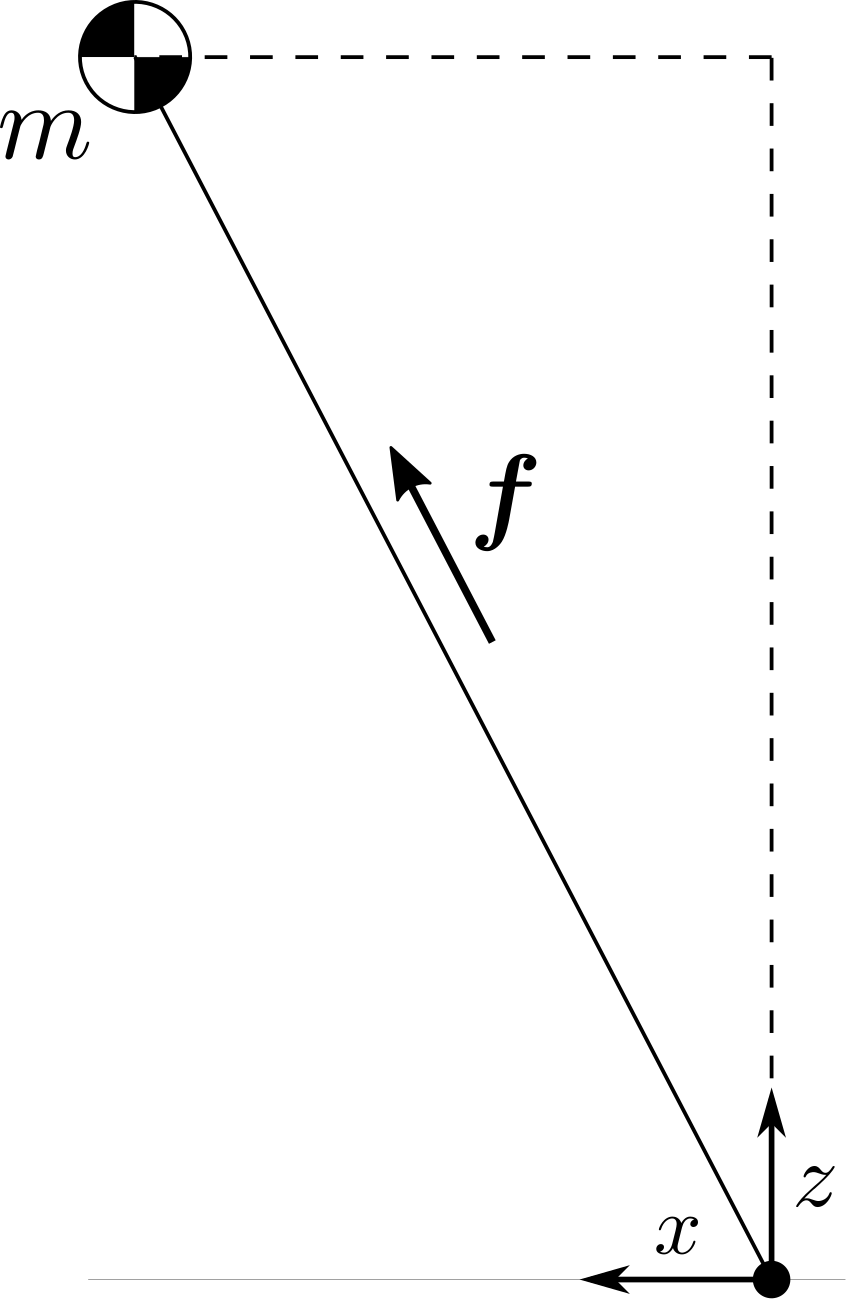
\includegraphics[width=0.25\textwidth]{STYLESTUFF/2Dnonlin.png}
\caption{Nonlinear simplified system in \ac{2D}.}
\label{fig:2dnonlin}
\end{figure} 

The non-linear model of a traveling \ac{CoM} subject to a force coming from the $[0,0]$ point on the ground is for the \ac{2D} $xz$-plane
\begin{eqnarray}
m\ddot{x} = F \frac{x}{\sqrt{x^2+z^2}}\\
m\ddot{z} = -mg+F \frac{z}{\sqrt{x^2+z^2}}
\label{eq:nonlindyn}
\end{eqnarray} 
where $F=||\boldsymbol{f}||$ is the leg or ground reaction force and $[x,z]$ the position of the point mass.


\section{Orbital Energy for Nonlinear \ac{CoM} Trajectories}
The nonlinear equations of motion of Eq. \eqref{eq:nonlindyn} are used in \cite{pratt2007derivation}. The authors constrain $z=f(x)$ and integrate the equations of motion over time, how a similar conservation of orbital energy as in Eq. \eqref{eq:Elip} is derived. This orbital energy however is not required to be a straight line trajectory, but depends on the function $f(x)$. The  full integration can be found in the paper, but the final expression writes as
\begin{equation}
   E_{orbit} = \frac{1}{2}\dot{x}^2\bar{f}^2(x)+gx^2f(x) - 3g\int_{x_0}^xf(\xi)\xi d\xi = \frac{1}{2}\dot{x}_0^2\bar{f}^2(x_0)+gx_0^2f(x_0).
\end{equation}
where $\bar{f}(x)=f(x)-f'(x)x$, $[x_0,\dot{x}_0]$ is the initial horizontal state and velocity and $[x,\dot{x}]$ is the current horizontal state and velocity. There is experimented in simulation with a symmetric polynomial, where the trajectory is tracked using a PD feedback scheme where the leg force is the control input. The polynomial description makes the integral directly solvable, based on the initial and current state. To make a clear separation between \ac{Elip}, this energy form will be defined in this report as \ac{Eorbit}.\\
Recently, this is used in a \ac{MPC} formulation and basic simulations have been done in \cite{koolen2016balance}. The main idea in this paper is to define four constraints on the trajectory $f(x)$, which define the four constants of a cubic polynomial by a matrix inversion. Those consist of two constraints on the initial conditions, one constraint on the final condition and one constraint on the conservation of \ac{Eorbit}. The matrix inversion is done offline, so that the control input can directly be written as a function of the polynomial constants and thus as a function of the initial and final states. 

\section{\ac{DCM} for Varying Height}
A couple of attempts in the use of varying height are found in adaptations of the \ac{ICP}. A couple of variations on the \acf{DCM} are examples of this. There exist multiple definitions of this \ac{DCM} and for clarity different mentions are explained and compared, as some of them seem to be interesting with respect to height usage. For simplicity and comparability, in all coming equations the mentions of \ac{CoP} and \ac{ZMP} in the publications are set to zero. In \cite{takenaka2009real} the \ac{DCM} is defined as 
\begin{equation}
q = x + \frac{1}{\omega_0}\dot{x}
\label{eq:takenakadcm}
\end{equation} 
based on a \ac{LIP} model, where $[x,\dot{x}]$ is the \ac{CoM} position and velocity and $q$ is the \ac{DCM}. Thus, this point is the same as the \ac{ICP} from Eq. \eqref{eq:cp} plus the \ac{CoM} horizontal location. \\
In \cite{englsberger2013three} the \ac{DCM} is defined as a \ac{3D} point. This is used in a un-even terrain path planner. The \ac{DCM} is here defined as
\begin{equation}
\boldsymbol{\xi} = \boldsymbol{x} + b\boldsymbol{\dot{x}}
\label{eq:englsdcm}
\end{equation}
where $\boldsymbol{\xi}=[\xi_x,\xi_y,\xi_z]^T$ is the \ac{DCM}, $\boldsymbol{x}=[x_{CoM}, y_{CoM}, z_{CoM}]^T$ and $\boldsymbol{\dot{x}}=[\dot{x}_{CoM}, \dot{y}_{CoM}, \dot{z}_{CoM}]^T$ are the \ac{CoM} position and velocity and $b>0$ is the time-constant of the \ac{DCM} dynamics. \\
\cite{hopkins2014humanoid} uses this and defines the constant $b=1/\omega_0$, where $\omega_0=\sqrt{\frac{g}{z_{CoM}}}$. This makes it again the same as the \ac{ICP}, but with a $z$ component in the state. The \ac{DCM} is derived with respect to time, where $\omega$ is posed to be time varying, so the height is time varying. This brings a new expression and is called the time varying \ac{DCM}, where the derivative is written as
\begin{equation}
\boldsymbol{\dot{\xi}}=(1-\frac{\dot{\omega}}{\omega^2})\boldsymbol{\dot{x}}+\frac{1}{\omega}\boldsymbol{\ddot{x}}
\end{equation}
where $\omega$ is the so called time varying natural frequency of the inverted pendulum.\\
\cite{caron2018capturability} mentions it uses the \ac{DCM} from Takenaka et al. and writes this as 
\begin{equation}
\boldsymbol{\xi}(t) = \boldsymbol{\dot{c}}(t) + \omega(t)\boldsymbol{c}(t)
\label{eq:carondcm}
\end{equation}
if the \ac{CoP} vectors are set to zero, where $[\boldsymbol{c},\boldsymbol{\dot{c}}]$ is the \ac{3D} \ac{CoM} position and velocity and $\boldsymbol{\xi}$ is the \ac{3D} \ac{DCM}. This is used in a \ac{MPC} scheme to capture the inverted pendulum \ac{CoM}. There is stated that if $\omega$ is not time varying, $\omega=\sqrt{\frac{g}{z}}$ holds. As is stated in the paper that the \ac{DCM} of Eq. \eqref{eq:carondcm} is a velocity rather than a point, this is equal to the time derivative of Eq. \eqref{eq:englsdcm}.

\section{Other Approaches}
Besides derivations of the \ac{ICP} for varying height and the \ac{Eorbit}, there are other approaches that describe the effects of varying height. The authors of \cite{gao2017increase} come up with different strategies to use varying height to generate impact or to relatively speed up the \ac{CoM} motion compared to the \ac{ICP} trajectory. Besides gravity, an extra vertical acceleration constant is added in the \ac{LIP} equations of motion. \\
In \cite{liu2015trajectory} a so called \ac{SLIP} model is used to deal with height variation on a humanoid robot. The \ac{SLIP} model lets the pendulum behave like a spring, where a control gain $k$ accounts for the `stiffness' of the spring. Trajectories are generated using an optimization program.\\
An applied approach is described in \cite{nguyen2017dynamic}. For different step lengths and step heights, trajectories are generated offline using a direct collocation optimization framework. Online is interpolated between trajectories with knowledge of the current step and the upcoming step. The trajectories are on joint level and make use of the earlier discussed \ac{HZD} approach. This is applied on hardware, but with the sagittal motion supported and thus only the \ac{2D} dynamics in the $xz$-plane are considered. Interesting is that the different trajectories correspond with different step timings, which is not always implemented in humanoid robot motion planning.\\
In \cite{tedrake2010lqr} is an extensive method described to generate a motion plan for nonlinear systems. In an algorithm, Lyapunov functions of local linearizations of the nonlinear model are evaluated, from which a feasible trajectory is derived. The main idea is that with the Lyapunov functions a measure of convergence of the local system can be proved. From a set of regions defined by converging functions, a feasible trajectory can be selected. Experiments are done on an inverted pendulum, generating trajectories for the swing-up task.\\

\section{Trajectory Optimization for Nonlinear Systems}
As becomes clear, looking at the simplified varying height robot model, nonlinearity is one of the main bottlenecks. As such, it would be rewarding to have already an insight in trajectory optimization for such systems. \cite{kelly2017introduction} poses a MATLAB  toolbox that can be used to solve trajectory optimization problems. In the toolbox an example can be found on the application of the algorithm on a simplified humanoid robot model. Furthermore, it gives a lot of information on how the solvers work. Nonlinear trajectory optimization methods distinguish themselves between direct and indirect methods, shooting and collocation methods and the difference between the so called `h'- and `p'-methods. The latter two define the degree of segmentation and the order of used functions between the segments of the problem. Direct collocation methods are most likely best suited for the subject of interest, as they require less computation time than indirect and shooting methods. Using the system description of Eq. \eqref{eq:nonlindyn}, a direct collocation method could be used for generating a nonlinear trajectory for example. 

\section{Analysis \& Discussion}
The discussed attempts to use varying \ac{CoM} height seem interesting, as they differ a lot from each other in how they are derived and used. The \ac{Eorbit} is used for both planning problems and for formulating a \ac{MPC} that uses varying leg force to come to a stop. By restriction of the $z$-coordinate to be a function of $x$, the equations of motion can be integrated in a similar way as in \ac{Elip}. This can now be used to relate height trajectories with respect to an ankle position with the state of the \ac{CoM}. In the \ac{MPC} approach, this is used to achieve the final goal of `capturing' the \ac{CoM} above the ankle. The virtual constraint of the function description assumes the direction of motion in $x$ does not change, which might in some cases be or be not be a problem. Another important aspect is that this derivation is done for the \ac{2D} side view case. As the authors of \cite{koolen2016balance} describe, virtual constraint approaches are best suited if the degree of underactuation is one. The degree of underactuation in this system is the number of degrees of freedom minus the number of inputs. This corresponds to the number of states minus the leg force, which equals one. In a \ac{3D} case integration of the equations of motion might be more challenging and also hard to use for implementation. \\
The \ac{DCM} approaches that consider height variation are interesting to make a more in-depth analysis as well. Assumed they all origin from the uncoupled \ac{2D} \ac{ICP} description and thus the \ac{LIP} orbital energy, a couple of things can be said. Considering the $z$-coordinate of the state of one of the \ac{3D} \ac{DCM} descriptions, for example Eq. \eqref{eq:englsdcm}, the dynamics in the vertical direction write as
\begin{equation}
\xi_z - z= \sqrt{\frac{z_0}{g}}\dot{z}.
\end{equation}
It rises questions if it is a good assumption that the vertical direction has the same dynamics as the \ac{ICP}. \\
Considering the time-varying \ac{DCM}'s $xy$-components, the \ac{ICP} and thus \ac{Elip} is derived with respect to time, where $z$ is posed to be time-varying. This might be a good approximation for the use in planning or control. Apart from this, with the integration of the \ac{LIP} equations of motion $z$ is already posed to be constant. The \ac{Elip} would look different, and $x$ and $z$ would be coupled, if $z$ would be time varying. 
The strategies described in \cite{gao2017increase} give a different perspective on the problem and are inspiring in the sense that also separate strategies can be evaluated, instead of solving a planning problem only. \\
\cite{liu2015trajectory} seems also an interesting approach. Possible concerns are the computation time of the optimization solver and the fact that a walking gait is generated without a predefined footstep plan.
The application of \cite{nguyen2017dynamic} gives an alternative method for real-time use, namely that of interpolating between precomputed libraries. Although the dynamics of the robot and the control framework used for it are quite different than those used at IHMC, it is an interesting approach to think about. The fact that the offline trajectories were generated using a direct collocation method, rises also the question if a direct collocation method would be fast enough for the use in a \ac{MPC} algorithm for example.\\